\begin{center}
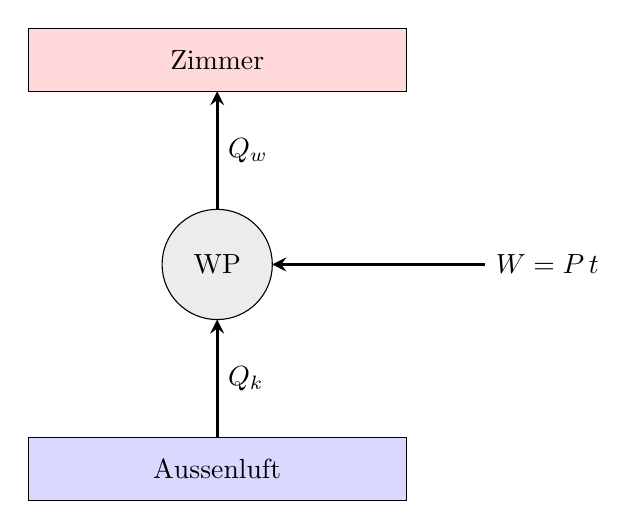
\begin{tikzpicture}[>=stealth]
 \draw[fill=red!15] (-2.4,2.2) rectangle (2.4,3.0);
 \node at (0,2.6) {Zimmer};
 \draw[fill=gray!15] (0,0) circle (0.7);
 \node at (0,0) {WP};
 \draw[fill=blue!15] (-2.4,-2.2) rectangle (2.4,-3.0);
 \node at (0,-2.6) {Aussenluft};
 \draw[->, very thick] (0,0.7) -- (0,2.2) node[midway, right] {$Q_\text{w}$};
 \draw[->, very thick] (0,-2.2) -- (0,-0.7) node[midway, right] {$Q_\text{k}$};
 \draw[->, very thick] (3.4,0) -- (0.7,0) node[pos=0, right] {$W = P\,t$};
\end{tikzpicture}
\end{center}

Die Leistungsziffer der Wärmepumpe ist das Verhältnis der ins Haus abgegebenen Wärme $Q_\text{w}$ zur aufgenommenen elektrischen Energie $W = P\,t$:
\begin{align}
 \eta_\text{WP} &= \frac{Q_\text{w}}{W}
\end{align}
Nach dem Energiesatz stammt $Q_\text{w} = W + Q_\text{k}$ aus der elektrischen Energie und der Wärme $Q_\text{k}$ aus der Aussenluft. Damit ist
\begin{align}
 Q_\text{k} &= Q_\text{w}-W = \QkF \\
   &= \left(\ewpO-1\right)\cdot\Pwp\cdot\tm \\
   &= \Qk \approx \result{\QkP{3}{2}}
\end{align}
